\chapter{Návrh architektury}

Aplikace je rozdělena na serverovou a klientskou část. Server slouží pro odstínění klienta od RDF databází, komunikuje tedy přímo s datovými zdroji a zpracovaná data předává klientské aplikaci. Klient pak v případě potřeby z internetu stahuje externí obrázky (příkladem jsou konfigurace Wikidat, které obsahují URL odkazy) a autocomplete soubory.

Rozdělení aplikace na klient-server také umožňuje cachování na straně serveru, které ještě implementováno není. Tento problém je diskutován v poslední kapitole.

\begin{figure}[h]
    \centering
    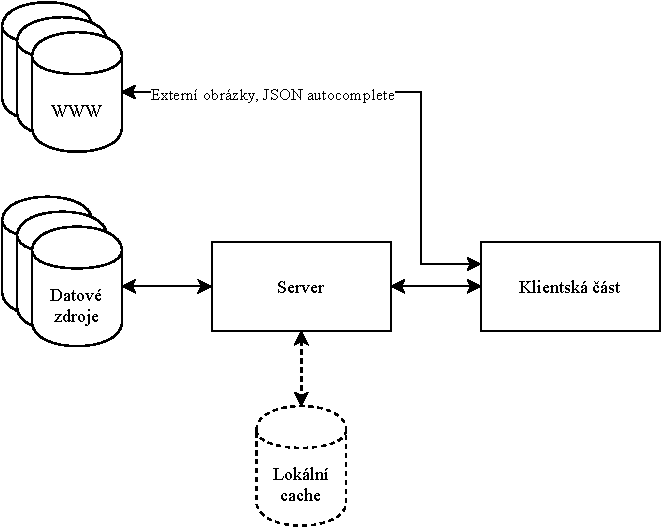
\includegraphics[width=0.75\textwidth]{media/communication.pdf}
    \caption{Komunikace mezi klientem, serverem a datovými zdroji. Cachování na serveru ještě implemontováno není.}
\end{figure}

\section{Server}
Jak již bylo v dokumentu zmíněno, převážná část serveru byla dodána jako specifikace pro klientskou aplikaci.

\subsection{Jazyková podpora} \label{jazykova-podpora}
Server jsem částečně přepsal, aby podporoval dotazování na data z více světových jazyků. Některé požadavky přijímají parametr \texttt{languages} obsahující čárkou (\texttt{,}) oddělené ISO 639-1 jazykové kódy. Server pak vrací objekty jejiž klíčem je jazykový kód a hodnotou daný překlad do jazyka. Pokud překlad neexistuje, hodnotou je \texttt{null}. V případě, že na všechny jazyky bylo vráceno \texttt{null}, server se pokusí přidat další jazyk, který existuje. Který jazyk takto bude vybrán není určeno.

Tato implementace umoňuje stahování vícejazyčných dat tak, že jsou stažené jen žádané jazyky, což může značně ušetřit přenos dat v některých případech, ale současně dojde ke stažení alespoň jednoho podporovaného jazyka, pokud je to možné.

\begin{prikl}
Pro \texttt{languages=cs,en} může server vrátit například
\begin{code}[frame=none]
{
    cs: null,
    en: "Kankakee County"
}
\end{code}
ale pokud nezná překlad ani do češtiny, ani do angličity, může vrátit
\begin{code}[frame=none]
{
    cs: null,
    en: null,
    sk: "Jazero Beňatina"
}
\end{code}
\end{prikl}

\subsection{API}
Server vrací data ve formátu JSON, požadavky jsou posílány metodou GET a parametry jsou kódovány do URL adresy.

\begin{figure}[p]
    \centering
    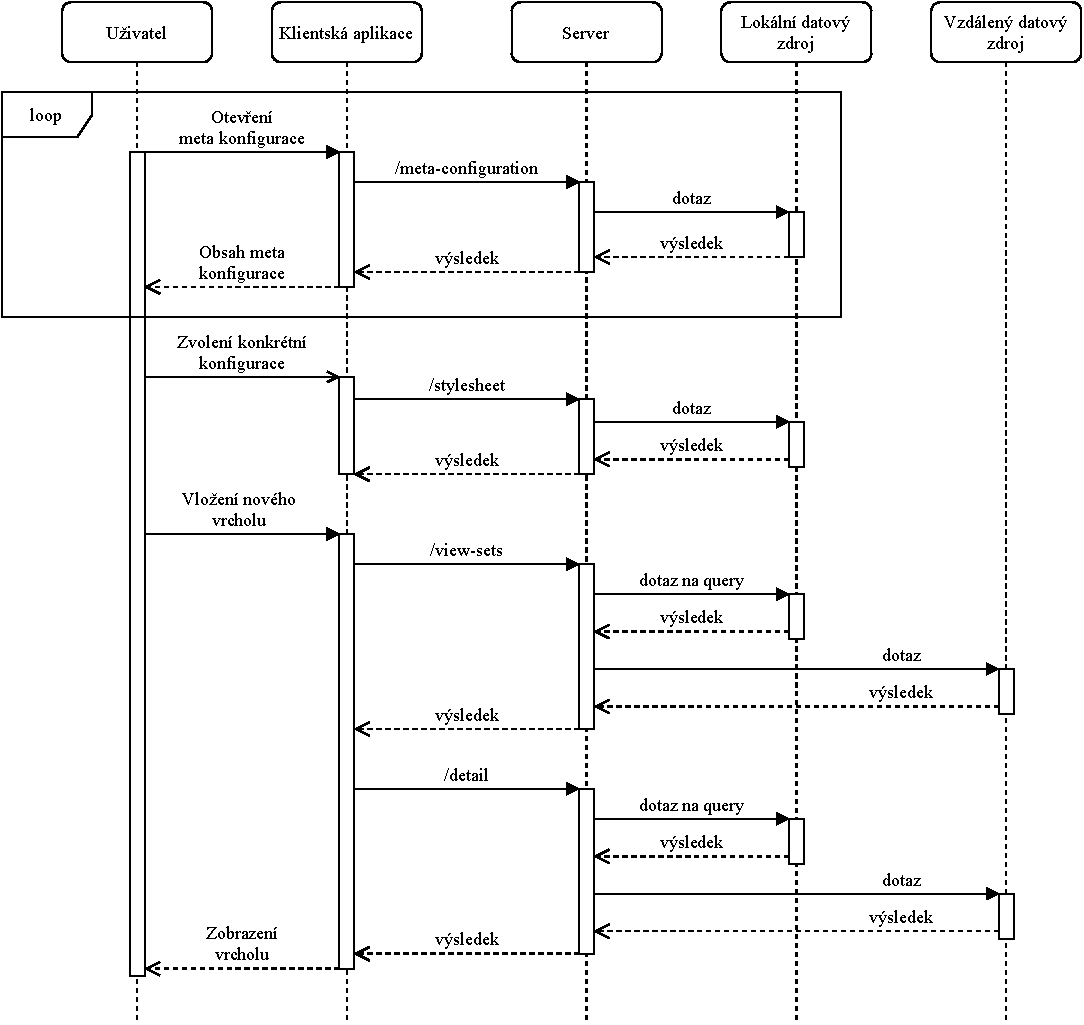
\includegraphics[width=\textwidth]{media/sequence-server.pdf}
    \caption{Schéma komunikace se serverem a RDF databází při spuštění aplikace. Nejprve klient vybírá konfiguraci. Poté začne stahování stylesheetu a stahování prvního vrcholu. Nejprve se stáhnout \texttt{view-sets} a poté z výchozího pohledu se stáhne \texttt{detail} a vrchol se zobrazí na grafu.}
\end{figure}

\subsubsection{/metaconfiguration}
\textbf{parametry:} \texttt{iri} a \texttt{languages} \\
Vrátí informace o metakonfiguraci zadané podle \texttt{iri}. \\
Vrátí všechna data (viz kapitola \ref{pozadavky-metakonfigurace}) o metakonfiguraci, veškerá data o dceřiných konfiguracích (viz kapitola \ref{pozadavky-konfigurace}) a základní data o dceřiných metakonfiguracích (vše kromě seznamu konfigurací a metakonfigurací).

\begin{code}
interface ResponseMetaConfiguration extends
ResponseMetaConfigurationBase {
    has_meta_configurations: ResponseMetaConfigurationBase[],
    has_configurations: ResponseConfiguration[],
}

interface ResponseMetaConfigurationBase {
    iri: string,
    title: {[language: string]: string},
    description: {[language: string]: string},
    image: string,
}
\end{code}

\subsubsection{/configuration}
\textbf{parametry:} \texttt{iri} a \texttt{languages} \\
Vrátí informace o konfiguraci zadané podle \texttt{iri}. \\
Vrátí stejná data jako \texttt{/metaconfiguration} o svých sceřiných konfiguracích. \\
Toto volání se používá pouze když uživatel ručně zvolí IRI konfigurace, v opačném případě si aplikace vystačí s voláním \texttt{/metaconfiguration}.

\begin{code}
interface ResponseConfiguration {
    iri: string,
    stylesheet: string[],
    title: {[language: string]: string},
    description: {[language: string]: string},
    autocomplete: string[],
    starting_node: string[],
    resource_pattern: string|null,
}
\end{code}

\subsubsection{/stylesheet}
\textbf{parametry:} \texttt{stylesheet} \\
Vrátí kompletní visual style sheet (viz kapitola \ref{pozadavky-visual-style-sheet}) na základě jeho IRI jako parametr \texttt{stylesheet}.

\begin{code}
interface ResponseStylesheet {
    styles: {
        selector: string;
        properties: {
            [property: string]: string;
        }
    }[];
}
\end{code}

\subsubsection{/view-sets}
\textbf{parametry:} \texttt{config} a \texttt{resource} \\
Vrátí seznam možných view setů (viz kapitola \ref{pozadavky-view-sets}) které odpovídají uzlu s IRI \texttt{resource} při dané konfiguraci \texttt{config}.

\begin{code}
interface ResponseViewSets {
    viewSets: {
        iri: string;
        label: string;
        defaultView: string;
        views: string[];
    }[];
    views: {
        iri: string;
        label: string;
    }[];
}
\end{code}

\subsubsection{/preview}
\textbf{parametry:} \texttt{view} a \texttt{resource} \\
Vrátí data z dotazu preview (viz kapitola \ref{pozadavky-preview}) na uzel s IRI \texttt{resource} při daném pohledu \texttt{view}.

\begin{code}
interface ResponsePreview {
    nodes: ResponseElementNode[];
    types: ResponseElementType[];
}
\end{code}

\subsubsection{/detail}
\textbf{parametry:} \texttt{view} a \texttt{resource} \\
Vrátí data z dotazu detail (viz kapitola \ref{pozadavky-detail}) na uzel s IRI \texttt{resource} při daném pohledu \texttt{view}.

\begin{code}
interface ResponseDetail {
    nodes: {
        iri: string;
        data: {
            [IRI: string]: string;
        };
    }[];
    types: ResponseElementType[];
}
\end{code}

\subsubsection{/expand}
\textbf{parametry:} \texttt{view} a \texttt{resource} \\
Vrátí expandované uzly (viz kapitola \ref{pozadavky-expansion}) pro uzel s IRI \texttt{resource} při daném pohledu \texttt{view}. Tyto expandované uzly již obsahují data o detailu a tedy není třeba žádného dalšího volání.

\begin{code}
interface ResponseExpand {
    nodes: ResponseElementNode[];
    edges: ResponseElementEdge[];
    types: ResponseElementType[];
}
\end{code}

\newpage

Mezi pomocná rozhraní pak patří
\begin{code}
interface ResponseElementType {
    iri: string;
    label: string;
    description: string;
}

interface ResponseElementEdge {
    source: string;
    target: string;
    type: string;
    classes: string[];
}

interface ResponseElementNode {
    iri: string;
    type: string;
    label: string;
    classes: string[];
}
\end{code}

\section{Klientská část aplikace}

\subsection{Moduly}

\begin{figure}
    \centering
    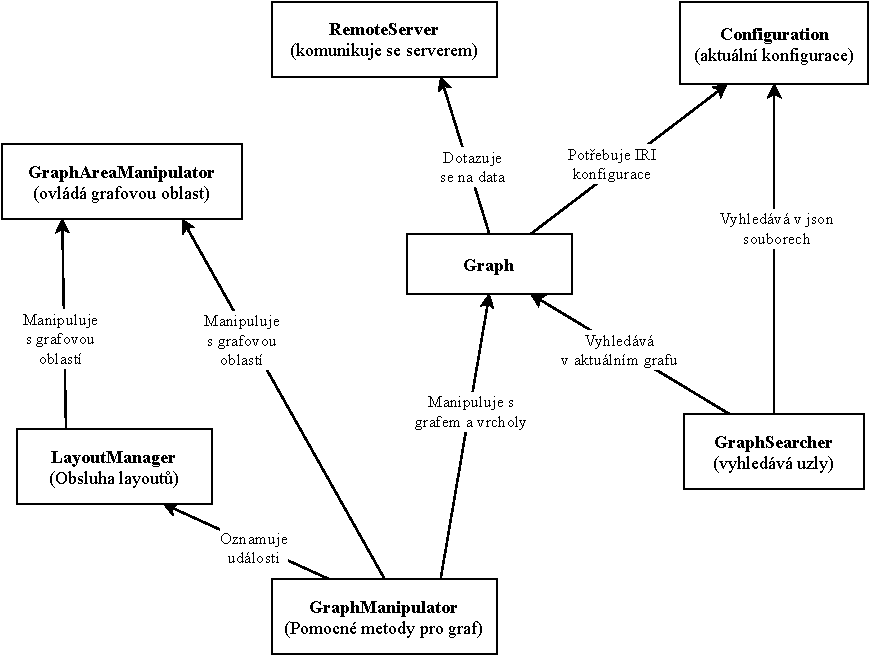
\includegraphics[width=\textwidth]{media/dependencies.pdf}
    \caption{Závislost modulů a dalších částí aplikace na sobě. \todo{Mohl bych se zeptat? Počítá se toto jako popis vazeb mezi moduly? Tento obrázek popisuje skutečné závislosti a používá skutečná jména tříd z aplikace. Můžu ho tedy v této části použít (i když ne vždy odpovídá textu v této kapitole), nebo ho mám dát k implementaci a tady dát něco jiného?}}
\end{figure}

Následující text popisuje rozvržení klientské části do modulů a jejich vzájemnou integraci.

\subsubsection{Připojení na server}
Modul řeší komunikaci se serverem. Obsahuje metody odpovídající API serveru, které vracejí data ve správném interface. V případě chyby vrátí jako odpověď false. Vyžaduje URL adresu serveru se kterým má komunikovat.

\subsubsection{Graf}
Tato část aplikace reprezentuje stažený graf a všechny jeho data. Má metody pro práci s grafem, jeho modifikaci a stahování nových dat ze serveru.

Využívá modul pro připojení na server.

\subsubsection{Práce s grafovou oblastí}
Tento modul odpovídá za práci s grafovou oblastí, tedy s plátnem, na které se vykresluje graf. Řeší manipulaci s grafovou oblastí, správné umístění nových vrcholů v rámci grafu a podobně.

Využívá modulu Graf pro práci s grafem.

\subsubsection{Filtrování}
Modul integruje možnost filtrování vrcholů v aplikaci na základě různých grafových a sémantických vlastností.

Obsahuje množinu filtrů, která může být za běhu aplikace měněna a tedy umožňuje aplikaci rozšířit o nové filtry pomocí pluginů. Každý filtr pak
\begin{itemize}
    \item Zodpovídá za vykreslení uživatelského rozhraní pro nastavení parametrů filtru.
    \item Má vlastní parametry
    \item Obsahuje třídu, která bude instanciována pro každý vrchol a na základě parametrů filtru a dat vrcholu rozhodne, zda je vrchol viditelný.
\end{itemize}

Filtrování tedy potřebuje přístup ke grafu.

\subsubsection{Layoutování}
Modul řeší uspořádání vrcholů v grafu, přičemž může reagovat na významné události grafu, jako přidání nového vrcholu, expanzi atp.

Obdobně jako filtrování, modul layoutování obsahuje množinu layoutů, která může být za běhu aplikace měněna. Každý layout pak
\begin{itemize}
    \item Zodpovídá za vykreslení uživatelského rozhraní pro nastavení parametrů layoutu.
    \item Má vlastní parametry
    \item Provádí layoutování, pokud je daný layout aktivní.
    \item Může vykreslit dodatečná tlačítka do uživatelského rozhraní pro snazší obsluhu layoutování.
\end{itemize}

Vždy je aktivní právě jeden layout. Pokud dojde ke změně layoutu, je o tom starý, i nový layout informován. Aktivní layout pak přijímá události z aplikace na které může reagovat. Využívá právě modulu práce s grafovou oblastí.

\subsubsection{Vyhledávání}
Modul vyhledávání vrací IRI vrcholy konfigurace na základě textového řetězce. Vyhledává v grafu, z autocomplete nebo se pokusí IRI sestavit z hledaného výrazu.

Modul má několik vyhledávačů a každý se pokusí na základě hledaného výrazu vrátit nalezené vrcholy. Ty jsou pak vhodně sloučeny a seřazeny do jednoho seznamu. Modul vyhledávání sám o sobě nezávisí na žádné jiné části aplikace, nicméně jednotlivé vyhledávače ano.

Některé vyhledávače můžou mít větší šanci nalézt vrchol, ale menší dodat k němu podrobné informace. Příkladem může být vyhledávač, který sestavuje IRI vrcholu z hledaného výrazu. V takovém případě je vyhledávač schopen poskytnout pouze IRI, nicméně jiný vyhledávač může vrchol znát, ale nemusel ho být schopen podle hledaného výrazu najít.

Proto vyhledávání probíhá ve dvou fázích. V první fázi se na základě hledaného řetězce sestaví množina IRI adres vrcholů. Ty jsou následně předány ve druhé fázi všem vyhledávačům, které se pak snaží doplnit informaci k těmto vrcholům, například jejich popisek. Protože vyhledávače mohou využívat internet, je třeba výsledky vhodně přepočítat kdykoli nějaký z vyhledávačů vrátí výsledek.

Postup vyhledávaní je následující
\begin{enumerate}
    \item Dotaž se všech vyhledávačů současně na IRI, která odpovídají hledanému výrazu.
    \item Když vyhledávač odpoví, přidej výsledná IRI k již nalezeným (od jiných vyhledávačů) v rámci daného hledaného výrazu.
    \item Dotaž se všech ostatních vyhledávačů současně na ty IRI, která byla do seznamu přidána poprvé.
    \item Když vyhledávač odpoví, přidej informace o daných vrcholech a aktualizuj vyhledávané výsledky.
\end{enumerate}

\subsubsection{Ukládání do souboru}
Řeší ukládání stavu aplikace do souboru a jeho následnou obnovu. Každý modul aplikace, konkrétně třídy, co nesou data, mají metody na serializaci a deserializaci jejich vnitřního stavu. Jednotlivé stavy jsou pak získány ze všech modulů a uloženy do souboru. Obdobně opačným způsobem se soubor načte a jednotlivé objekty popisující stavy jsou zpět rozdistribuovány po aplikaci na obnovení stavu.

\subsubsection{Uživatelské rozhraní}
\todo{Můžu to považovat za modul? Je to vlastně určitá část aplikace co něco dělá.}
Poskytuje uživateli informace o vrcholech a umožňuje mu interagovat s grafem.